%\documentclass[english]{uzhpub}
\documentclass[12pt]{article}
\usepackage[T1]{fontenc}
\usepackage[latin9]{inputenc}
\usepackage{listings}
\usepackage{color}
\usepackage{longtable}
\usepackage{url}
\usepackage{graphicx}

\begin{document}



%% Titelei
\title{Master Project: Clustermeister}

%\subtitle{Report}

\author{Daniel Spicar, Thomas Ritter}

\date{\today}

\maketitle

\definecolor{lbcolor}{rgb}{0.9,0.9,0.9}
\definecolor{white}{rgb}{1.0,1.0,1.0}

\section{Motivation}

Programming distributed systems poses a number of challenges for a developer. One of these challenges is to request, configure and start a distributed computing infrastructure. This is the problem of provisioning. Another challenge is to package, deploy and run code on the distributed computing infrastructure. This is the problem of deployment and execution. Clustermeister has been made to support Java/Scala developers in tackling this challenge by providing dynamic provisioning and deployment in cloud and cluster computation environments.

Dynamic provisioning means that with Clustermeister a developer can set up a distributed computation environment, and then alter it at any time during a session. In Clustermeister terminology a developer can add and remove nodes and shut the environment down again. A node is an addressable unit that can execute code. Clustermeister abstracts the underlying specifics of the computation environment from the user. This way multiple environment can be supported and the user does not have to maintain various tools and scripts and interact with different APIs.

Dynamic deployment means that Clustermeister can deploy new and changed code to nodes without the need to interact with the distributed computation environment manually. This means a developer can just run changed code and does not need to worry about updating and restarting code deployments in the distributed environment. This can save a lot time and hassle when developing a distributed system.

Provisioning and deployment are tasks that interact with distributed computation environments and this is handled transparently to the user by the Clustermeister Provisioning module. Code execution on the other hand must interact closely with user code. For this purpose the Clustermeister API forms a bridge between the infrastructure provided by Clustermeister and the user code. The API offers various methods for code execution. Some allow to address specific nodes, others will distribute tasks to available nodes transparently.

The aim of the project is to support developers by letting them concentrate on their code and solve infrastructure challenges reliably and with minimal configuration.

\subsection*{Clustermeister provides:}
\begin{itemize}
\item Dynamic distributed computation infrastructure provisioning.
\item Dynamic class-loading allowing for client code execution without manual re-deployment.
\item Easy deployment of dependencies using Apache Maven dependency resolution.
\item Parallel and distributed code execution via a Java ExecutorService interface or a native inferface.
\item Addressable nodes for code execution on specific nodes.
\item Provisioning of Amazon Web Services Elastic Compute Cloud (EC2) and TORQUE (PBS) infrastructure.
\end{itemize}

\section{Evaluation of Third-Party Libraries}

Java was chosen as the platform for Clustermeister, because it was known that Clustermeister will be used by Scala clients, so the JVM was a logical decision. Another goal was to licence Clustermeister under the Apache Licence, version 2.0. These were the two most important constraints while searching for suitable libraries.

The goal for Clustermeister was not to re-implement a node runtime based on Java, so instead existing libraries were evaluated that would help to run code on remote JVMs. Ideally, this runtime should provide a means of dynamically loading libraries and classes from the machine that is issuing the computation task.

There are a few libraries that would fit the needs. We selected three libraries to evaluate. These are 
GridGain\footnote{http://www.gridgain.com/}, 
Hazelcast\footnote{http://www.hazelcast.com/} and 
JPPF\footnote{http://jppf.org/}. In the following, these libraries and their characteristics are discussed.

\paragraph{GridGain} GridGain was very easy to set up, has a pleasant API and worked out of the box. It is able to remotely load libraries and classes without additional configuration. However, newer versions of GridGain are licenced under the GPL. Further, there was no obvious way to configure GridGain programmatically. Because of these reasons, GridGain was ruled out.

\paragraph{Hazelcast} Hazelcast was a good fit at first sight, due to its nice API. However, it lacked features that were needed for Clustermeister, i.e. remote deployment of libraries and classes and provisioning capabilities. Hazelcast is generally a low-level solution and it would have required more implementation effort to integrate it into Clustermeister.

\paragraph{JPPF} JPPF was a good fit for the requirements. It is licenced under the Apache Licence and is being actively developed. Further, there is good community support and it fits the needs for Clustermeister. Therefore, JPPF was chosen to build the basic infrastructure.

\section{Architecture and Specification}
\label{architecture}

In this section, Clustermeister's high-level architecture is characterized. First, Clustermeister terminology is introduced. Second, the most important building blocks and modules are presented. At the end of this section, the Clustermeister topology is explained with an example set-up.

\subsection{Terminology}

\begin{description}
\item[Clustermeister Node] A node can be interpreted as a JVM that executes code. Nodes are running on local or remote Clustermeister instances. A single instance can host several nodes.
\item[Clustermeister Instance] An instance is a physical or virtual machine generally running in a cluster or a cloud computation service such as Amazon EC2.
\end{description}

\subsection{Use Cases}

\subsubsection*{Abstract Use Case}
This abstract use case that has been compiled from the project definition and discussion among the developers and the project leadership. It aims to demonstrate how Clustermeister can be used in a development workflow. The use case applies to Java and Scala developers.

\begin{enumerate}
\item \label{uc:start}The developer begins a programming session.
\item The developer starts Clustermeister locally from the command line.
\item \label{uc:alloc}Using the terminal where Clustermeister is running, the developer allocates five Clustermeister nodes in a distributed computation infrastructure.
\item \label{uc:prog}The developer programs a parallel algorithm and uses the Clustermeister API in the source code to submit parallel tasks to the Clustermeister nodes requested in step \ref{uc:alloc}.
\item The developer compiles the code and executes it. The result is not as expected.
\item The developer corrects a bug in the source code, re-compiles it and executes it again. This time the result is correct.
\item The developer wants to speed up the computation. He opens the terminal where Clustermeister is running and requests another five Clustermeister nodes.
\item The developer executes his program again, without re-compilation. This time the result has been computed faster.
\item The developer is satisfied with the result and de-allocates all Clustermeister nodes using the terminal where Clustermeister is running.
\item The programming session ends.
\end{enumerate}

\subsubsection*{Specific Use Cases}
There are many specific use cases that can be derived from this abstract use case. Here are examples of specific variations that will be supported:

\begin{description}
\item[Step \ref{uc:start}.1] The developer wants to execute some code in a distributed manner, not planning to do any development.
\item[Step \ref{uc:alloc}.1] The developer allocates five nodes in the Amazon Web Services Elastic Compute Cloud (EC2).
\item[Step \ref{uc:alloc}.2] The developer allocates five nodes in the TORQUE Cluster provided at the department of informatics in the University of Zurich.
\item[Step \ref{uc:prog}.1] The developer programs a distributed AKKA\footnote{http://akka.io/} actor system. The Clustermeister API allows to iterate through available nodes and bootstrap an actor system by submitting actors to the nodes for execution.
\end{description}

\subsection{Specification}
In the project definition the following requirements relevant for the architecture have been identified:

\begin{enumerate}
\item A method of querying the state of the provisioned infrastructure (Clustermeister nodes) must be available in Clustermeister.
\item A method of adding and removing nodes to or from the provisioned infrastructure must be available in Clustermeister.
\item Clustermeister must offer an API that can be used from Java and Scala and enables user code to interact with Clustermeister nodes. The API must offer:
\begin{enumerate}
\item Access to a Java collection describing all available nodes.
\item Nodes offer a method to submit code to them for execution.
\end{enumerate}
\item Changed code needs to be deployed and loaded on the nodes automatically.
\item The communication with the cluster nodes should be secured and require some form of authorization. 
\end{enumerate}

\subsection{Architecture}

\subsubsection{Clustermeister Modules}

Clustermeister consists of two main modules: Provisioning and API.

Clustermeister Provisioning is running in an independent user process on the developer's machine and implements the Clustermeister API.

The Clustermeister API is a library that can be used in user code in order to interact with Clustermeister Provisioning. 

This separation of concerns enables the user to set up and deploy Clustermeister nodes at the beginning of a session and then change and execute code repeatedly, without the need to perform any manual re-deployment. This speeds up developing and testing code in a distributed environment.

\subsubsection{Clustermeister Provisioning}
The provisioning module is accessible via a command line interface (CLI) and is responsible for deployment of the Clustermeister infrastructure. This enables provisioning of instances and nodes, deployment of dependencies and dynamic classloading.

Provisioning is the core of Clustermeister's dynamic code deployment and execution `magic' and implements the specifics of interacting with supported cloud or cluster computation infrastructures.

\subsubsection{The Clustermeister API}
Allows the user to send jobs and tasks to Clustermeister nodes for execution and access to the computation's results. The computations are executed asynchronously, in parallel and in a distributed manner. Clustermeister API supports execution of Serializable and Java code. This does not exclude code written in other, bytecode compatible, programming languages such as Scala.

\subsection{JPPF}

JPPF is a client-server based framework/library written in Java. JPPF nodes connect to a JPPF server (also called driver) and receive tasks which they execute. A JPPF server may connect to a parent server and acts as a node to receive tasks. In a Clustermeister setup, a local JPPF server is always started. Nodes in a Torque cluster or on an Amazon instance connect to this local JPPF server. Code that is executed via the Clustermeister API connects to the local JPPF server and the server distributes the tasks to the connected nodes.

\subsection{Toplology}
\label{topology}

\begin{figure}[h]
\centering
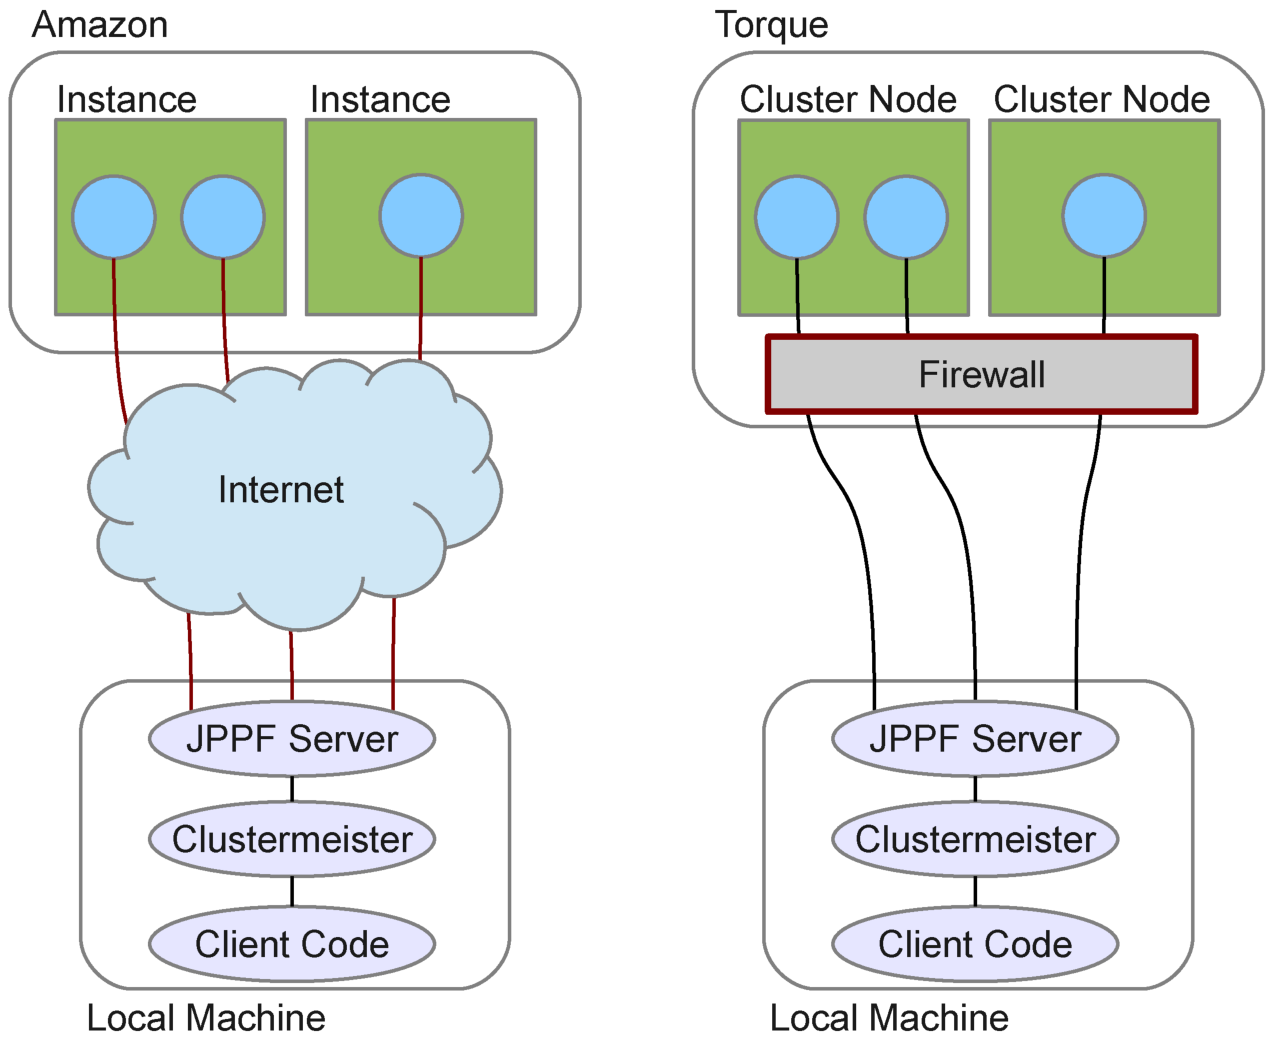
\includegraphics[scale=0.5]{images/topology.pdf}
\caption{Topology}
\label{fig:topology}
\end{figure}

Fig. \ref{fig:topology} depicts a high-level view on a typical Clustermeister topology.

On the left side, you can see a Clustermeister setup for Amazon EC2. In this case, two instances are provisioned. There are two Clustermeister nodes running on the first instance, and one node running on the second instance. Each node uses an SSH tunnel to the local machine to connect to the JPPF server. The local JPPF server is started by Clustermeister automatically once the command-line client is started. Nodes provisioned on Amazon instances connect to this server via SSH tunnels automatically. Once they are connected, end-users are able to use them via the Clustermeister API. The Clustermeister API communicates with the local JPPF server and the server manages and distributes computation tasks.

On the right side, a set-up for Torque is depicted. The local part is the same as seen in the Amazon example, but there are a few differences otherwise. There is no direct access to the Torque cluster nodes themselves. The nodes are started on a job submission server (not in the picture) and the Torque infrastructure decides on which Torque cluster node Clustermeister nodes are started. Once a Clustermeister node is started, it connects to the JPPF server on the local machine. The Torque cluster firewall allows for outgoing traffic but does not allow for incoming traffic. The details are discussed in Sect. \ref{implementation-torque}.

\section{Implementation}
\label{implementation}

In this section, the Clustermeister implementation is discussed in detail and differences with regard to the implementation between the two target platforms, Amazon EC2 and Torque/PBS, are explained.

\subsection{Project Structure}
\label{structure}

Clustermeister uses Maven\footnote{http://maven.apache.org/} to manage dependencies and build artifacts. It is hierarchically organized with a parent \texttt{pom.xml} and several sub-modules:

\begin{itemize}
 \item \textbf{api}: this module contains the end-user visible parts of Clustermeister, i.e. its API and interfaces.
 \item \textbf{provisioning}: in this module, Amazon and Torque provisioning is implemented, as well as a general-purpose interface to allow for alternate provisioning targets
 \item \textbf{cli}: this is a relatively small module that provides a command line interface for node provisioning. It is basically a command-line frontend to the provisioning module.
 \item \textbf{driver}: this module is used to build an executable JPPF driver (server). It contains a few extensions for the original JPPF driver.
 \item \textbf{node-common}: this contains code that is used by both the (JPPF) driver and node module and can be seen as a ``shared library''.
 \item \textbf{node}: this module is used to build an executable JPPF node. It contains a few extensions for the original JPPF node to allow for special maintenance tasks.
 \item \textbf{integration-tests}: this module contains test ``scenarios'' written in Java as well as Scala that uses the Clustermeister API. These are tests that exercise the whole Clustermeister library.
\end{itemize}

\subsection{Module Dependencies}
In order to prevent to prevent dependency cycles and to understand node deployment, one must understand how Clustermeister modules depend on each other. In section \ref{structure} the modules have been described. This section relates them to each other.

The dependencies are depicted in Fig. \ref{fig:deps} for reference. Conceptually there are two rows of dependencies. The first row consist of modules that users of Clustermeister will work with. The second row consist of modules that are used to run Clustermeister nodes and drivers. It is very important to prevent any dependencies from the second row onto the first because all dependencies (direct and indirect) of the Node module must be deployed on Clustermeister instances and this should be minimized. Additionally there is a high likelihood of creating cyclic dependencies when introducing such dependencies. Currently drivers are only deployed locally but it is possible that Drivers will be deployed to instances as well in the future. The corresponding functionality is present in the Amazon provider. 

The CLI contains the entry point to the Clustermeister process and is compiled into an executable. Therefore nothing else should depend on it. The CLI depends on the driver module, because it launches a local driver to send jobs to distributed nodes. On the other end, there is the API module which should depend on as little as possible because it is used as a library in user-code and should not create too many additional dependencies. Provisioning depends on driver and node, because it deploys their compiled JAR packages to Clustermeister instances. It also uses code from node-common for node management.

\subsubsection{API Module Dependencies}
This is a listing to the direct dependencies of the API module. Users of the Clustermeister API need to provide these dependencies and their indirect dependencies at runtime.

\begin{itemize}
 \item snakeyaml (1.10)
 \item Apache Commons Configuration (1.8)
 \item jmxremote\_optional
 \item Google Guava (11.0.1)
 \item JPPF Server (3.1.1)
 \item JPPF Common (3.1.1)
 \item JPPF Common Node (3.1.1)
 \item JPPF Client (3.1.1)
\end{itemize} 

\subsubsection{Node Runtime Dependencies}
This is a listing to the runtime dependencies of the Node module. It is important to understand that these dependencies need to be deployed to Clustermeister instances and made available in the classpath of nodes. Clustermeister should handle this automatically but this serves to document the requirements as a reference when debugging or developing Clustermeister.

\begin{itemize}
 \item Clustermeister Node-Common (0.1-SNAPSHOT)
 \item JPPF Common Node (3.1.1)
 \item Log4J (1.2.16)
 \item SLF4J API (1.6.4)
 \item SLF4J Log4J Bindings (slf4j-log4j12 1.6.4)
 \item jmxremote\_optional
\end{itemize}

\begin{figure}[hp]
\centering
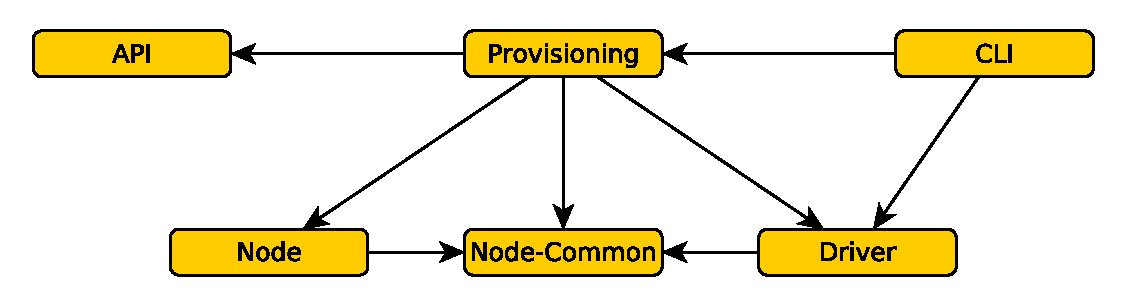
\includegraphics[scale=0.7]{images/module-deps.pdf}
\caption{Clustermeister module dependnecies. The arrows illustrate depends-on relationships. The dependencies are conceptually assigned into two rows. The first row consists of CLI, Provisioning and API. The second row consists of Driver, Node and Node-Common.}
\label{fig:deps}
\end{figure}

\subsection{API}

JPPF offers its own API as ``JPPF client''. Clustermeister uses the JPPF client to connect to the local JPPF driver and to send jobs internally. However, Clustermeister wraps this JPPF client with its own API that simplifies job execution and reduces the configuration to a minimum. To achieve this, Clustermeister offers its own job and task interfaces. However, the Clustermeister API permits access to the JPPF native API, if more control over job execution is desired. Further, it offers a Java \texttt{ExecutorService} that is inherited from the JPPF client API.

The Clustermeister API and its interfaces are designed to reduce configuration as much as possible, but some configuration is still necessary. In section \ref{configuration} the configuration options are discussed in detail.

JPPF Client that connects to local driver
+ custom Job/Task classes, access to native API, ExecutorService
+ Configuration?

interface to distributed infrastructure from user code

\subsection{Provisioning and Deployment}
Most of Clustermeister's functionality is implemented in the provisioning module. This module is responsible to start and manage Clustermeister nodes and make them available to users of the Clustermeister API. Because Clustermeister uses JPPF internally, the provisioning module is conceptually a JPPF driver (server) process that runs on the local developer's machine. The Clustermeister API connects to this server and sends jobs to it. The server itself maintains connections to the distributed nodes and, depending the load balancing strategy configured, distributes tasks to the available nodes. JPPF also solves the problem of dynamic classloading. Therefore, most of this module's code manages deployment of a JPPF setup in different environments. It also provides a number of utilities that support this task or improve the user experience.

- dep preloading impl. with aether
- SSH impl with jsch
- Amazon with jclouds, parallel
- Torque qsub...
- remote logging

\subsubsection{The Provisioning Process}
The provisioning process is started from the command line interface (CLI) and then creates a local JPPF driver process (see section \ref{localdriver}) and RMI servers for inter process communication (IPC) with the local driver process and the API (see \textit{RmiInfrastructure}, \textit{RmiServerForDriver} and \textit{RmiServerForApi}).

\subsubsection{The Local JPPF Driver Process}
\label{localdriver}
The local driver is implemented primarily in \textit{JPPFLocalDriver} and \textit{LocalDriverBuilder}. However, JPPF does not provide interfaces to communicate with this process. Therefore the local driver communicates with an RMI server (\textit{RmiServerForDriver}, \textit{CMNodeConnectionListener}) in the provisioning process, in order to inform it about changes in the JPPF environment (primarily node connections or disconnections).

\subsubsection{Node Management}

Node management refers to tasks such as starting or stopping nodes or gathering information about them. Clustermeister customized JPPF nodes such that they can perform such tasks when they receive special kinds of computation jobs. This was implemented this way because JPPF performs such management via JMX\footnote{http://www.oracle.com/technetwork/java/javase/tech/javamanagement-140525.html}, but distributing JMX is problematic with the licensing chosen for Clustermeister and it turned out not to be very reliable. The node management is primarily implemented in \textit{JPPFManagementByJobsClient}, which is a wrapper around a standard JPPF client. The different provider implementations (see section \ref{deployment}) can then create and use these clients to manage the node state or gather information about the nodes.

\subsubsection{Node Deployment}
\label{deployment}
lala

\paragraph{Torque Provider}

\label{implementation-torque}

Torque offers a generally static infrastructure for deployment. Computations tasks are started from a job submission machine that is accessed via SSH and Torque users have SSH access to this machine.

When accessed via SSH, Torque jobs are submitted with the \texttt{qsub} command. In Clustermeister, the job submission machine is accessed via SSH, then artifacts are uploaded and each node is started as a separate \texttt{qsub} job submission. Depending on how many CPU cores are requested for each job and how many jobs are issued by other participants, these nodes are started immediately or they may be queued. This is one of the difficulties involved with Torque, as node startups cannot be directly controlled.

Another difficulty is network access to nodes. A Torque cluster network is commonly isolated, therefore nodes are allowed to initiate connections, even to resources outside of the local network, but the nodes themselves are not accessible from outside. These constraints lead to difficulties in node management, because the JPPF node management infrastrucure relies on JMX and requires a direct connection to the node. Clustermeister circumvented this problem by extending the JPPF node runtime with management job extensions. These jobs are submitted equally to common computation tasks, but contain meta-data that is handled by the nodes. For example, if a node needs to be shut down, Clustermeister issues a special task and nodes react on it. These special tasks are not dynamic and need to be integrated before the node runtime is deployed. Therefore management tasks cannot be changed or installed while the node is running.

\subsubsection{Amazon}
The Amazon provider component manages Amazon EC2 instances and deploys JPPF nodes on them. The Amazon EC2 service offers many options for customizing and running instances. Clustermeister relies on the jClouds\footnote{http://www.jclouds.org/} library to interact with the EC2 API. It has been chosen because it supports all required features, is well maintained and offers its own API which is not specific to the underlying cloud computation service. This allows to extend Clustermeister with support for other services in the future.

The Amazon provider has been implemented such that it is able to build complex JPPF topologies\footnote{http://www.jppf.org/doc/v3/index.php?title=JPPF\_Overview\#Architecture\_and\_topology} \footnote{http://www.jroller.com/jppf/entry/master\_worker\_or\_p2p\_grid}. This means it can deploy arbitrary numbers of JPPF nodes and servers to any EC2 instance. However bugs in JPPF prevented this functionality to be fully active in Clustermeister. Therefore the provider supports the topology described in section \ref{topology} only

\subsubsection{Utilities}

\begin{description}
 \item[SSH] Both provisioning targets use jsch\footnote{http://www.jcraft.com/jsch/} for SSH access. However, the Amazon target uses jsch via the jclouds API, because jsch is integrated with jclouds. Further, nodes on Amazon instances use a reverse SSH tunnel to connect to the JPPF driver on the local machine.
 \item[Dependency Preloading] In the configuration file, the end-user can configure a pom.xml file or custom entries for dependencies that should be deployed to the node. This is implemented with the aether\footnote{http://www.sonatype.org/aether} library. For more information on how to configure this, see section \ref{appendix-general-configuration}.
 \item[Remote Logging] Logging output from (remote) nodes can be redirected to the local machine. This feature is implemented with log4j remote logging.
\end{description}


\subsection{CLI}

The CLI (command line interface) is a user interface for provisioning and can be seen as a front-end for the provisioning module. The command line interface contains a simple shell that allows to execute commands. The shell itself is implemented with the jline\footnote{http://jline.sourceforge.net/} library, which handles console input and offers features like command auto completion and a history mechanism.

A guide on how to use the command line interface can be found in section \ref{tutorial}.

jlines -> command completion
config loading
user interface for provisioning

\subsection{Node and Driver}
The node and driver module's main purpose is to wrap JPPF nodes and drivers to introduce custom functionality and to build self-contained zip archives that include their executables, static configuration files and their runtime dependencies. These archives can then be deployed by the provisioning module to Clustermeister instances, unpacked, and executed.

The customizations made include:

\begin{itemize}
\item Custom launchers that can launch nodes in different modes and with custom parameters to adjust functionality depending on the environment they run it (Amazon EC2 instance, Torque or the local machine). The main purpose is to redirect standard I/O streams and to adapt the process model to the environment's requirements.
\item Code to implement management job functionality (e.g. shut down the node upon receiving a special kind of job) is implemented in \textit{ClustermeisterNodeLifeCycleListener}.
\item When the driver is the local driver (see section \ref{topology}), it starts corresponding RMI infrastructure to communicate node connection events with the provisioning process.
\end{itemize}

\section{Organisation}

The project duration has been scheduled to three and a half to maximum four months and there has been no pre-existing code base to work from. The project team consisted of two students that worked approximately three days a week on the project. The project definition contained some organizational specifications for the Clustermeister project. Namely that the project shall be licensed under the Apache License, Version 2.0\footnote{http://www.apache.org/licenses/LICENSE-2.0.html}, developed on GitHub\footnote{https://github.com/} and make use of github's issue management and documentation facilities. Therefore Clustermeister is an open source project and all source code and documentation is publicly available at: \url{https://github.com/nethad/clustermeister}.

Given these specifications a number of coarse work items were identified:
\begin{enumerate}
\item \label{wi:spec}Specify the desired system's architecture and functionality (refer to section \ref{architecture} for more information).
\item \label{wi:res}Research and evaluate existing frameworks and libraries for re-use in this project. Particularly frameworks for parallel code execution in distributed JVMs.
\item \label{wi:fam}Familiarize with the desired target computation environments, Amazon Web Services Elastic Compute Cloud (EC2) and TORQUE (PBS).
\item \label{wi:impl}Implementation of the system (refer to section \ref{implementation} for more information).
\item \label{wi:eval}Testing and Evaluation of the solution.
\end{enumerate}

\subsection{Schedule}

The project team estimated the time necessary to spend on each work item and then defined a schedule (see Tab. \ref{tab:schedule}). Work items \ref{wi:res} and \ref{wi:fam} are included in the phase \emph{Evaluation} in the first three weeks. This phase should result in choosing a viable framework for the solution. Next the phase \emph{Implementation 1} follows, which contains the specification and architecture of the solution (work item \ref{wi:spec}) and focuses on implementation of the provisioning module (part of work item \ref{wi:impl}). The provisioning module is a critical centrepiece of the project. In week 10 it the evaluation of the performance of the provisioning module should become a focus (phase \emph{Evaluation 1}, part of work item \ref{wi:eval}). This does not mean that no tests are run before, but that week focuses on identifying critical problems before it is too late to repair them. The phase \emph{Implementation 2} gives opportunity to correct problems and implement the API (work items \
ref{wi:impl}). The last weeks (\emph{Evaluation 2}) should then focus on evaluating the complete system (work item \ref{wi:eval}) and correcting bugs (\ref{wi:impl}). The schedule is not to be interpreted as a definitive work plan in the style of the waterfall model\footnote{http://en.wikipedia.org/wiki/Waterfall\_model}. It associates to each week of the planned project duration the primary type of work that should be performed. For example: In the fifth week the project team will start work on the implementation of the Amazon EC2 provisioning module. The schedule then allows to identify how progress in the project is developing and if the project is on schedule or if action needs to be taken to be able to finish on time. That does not mean that in the fifth week work is restricted to the Amazon EC2 provisioning module, nor that no work is done on the EC2 module in other weeks.

\begin{table}[hptb]
\centering
\begin{tabular}{|l|l|p{7cm}|}
\hline
\textbf{Week} & \textbf{Phase} & \textbf{Major Tasks} \\ \hline
30.1. - 5.2. & Evaluation & JPPF, GridGain, Hazlecast, jClouds \\ \hline
6.2. - 12.2. & Evaluation & Prototyping with JPPF, Amazon EC2, Torque \\ \hline
13.2. - 19.2. & Evaluation & Prototyping Torque, Evaluation Wirr, JPPF Ext. features \\ \hline
20.2. - 26.2. & Implementation 1 & Provisioning: Architecture, API: Architecture \\ \hline
27.2. - 4.3. & Implementation 1 & Provisioning: Amazon \\ \hline
5.3. - 11.3. & Implementation 1 & Provisioning: Amazon \\ \hline
12.3. - 18.3. & Implementation 1 & Provisioning: Torque \\ \hline
19.3. - 25.3. & Implementation 1 & Provisioning: Torque \\ \hline
26.3. - 1.4. & Implementation 1 & Reserved \\ \hline
2.4. - 8.4. & Evaluation 1 & Run first Performance/Scalability Tests \\ \hline
9.4. - 15.4. & Implementation 2 & Implement Lessons Learned from Evaluation \\ \hline
16.4. - 22.4. & Implementation 2 & Implement Lessons Learned from Evaluation \\ \hline
23.4. - 29.4. & Implementation 2 & API \\ \hline
30.4. - 6.5. & Implementation 2 & API \\ \hline
7.5. - 13.5. & Implementation 2 & Reserved \\ \hline
14.5. - 20.5. & Evaluation 2 &  \\ \hline
21.5. - 27.5. & Evaluation 2 &  \\ \hline
28.5. - 3.6. & Evaluation 2 &  \\ \hline
\end{tabular}
\caption{Project Schedule.}
\label{tab:schedule}
\end{table}

\subsection{Working Methodology}

The two students worked on the project in a co-located environment. Since this was a small team, organization was often informally agreed upon. While responsibility for different parts of the system were split (e.g. between Amazon EC2 and Torque modules) they worked as a team, sometimes employing techniques such as code review or pair programming. In general the work methodology followed the ideas of agile software development\footnote{http://en.wikipedia.org/wiki/Agile\_software\_development} and iterative development. When starting work on a scheduled work item, the task was split into numbered \emph{Issues} that captured a confined unit of work (see Fig. \ref{fig:issues}). Issues have been worked on one at a time. This helped with the intention to avoid putting the code base into an inconsistent state because an issue could only be completed when it was properly implemented and tested. While the methodology did not necessarily follow the approach of test driven development\footnote{http://www.agiledata.
org/essays/tdd.html}, great effort was taken to write unit tests for most of the system in order 
to verify functionality in isolation. Additionally a small framework for integration tests has been written to ensure the solutions overall health.

\begin{figure}[hptb]
\centering
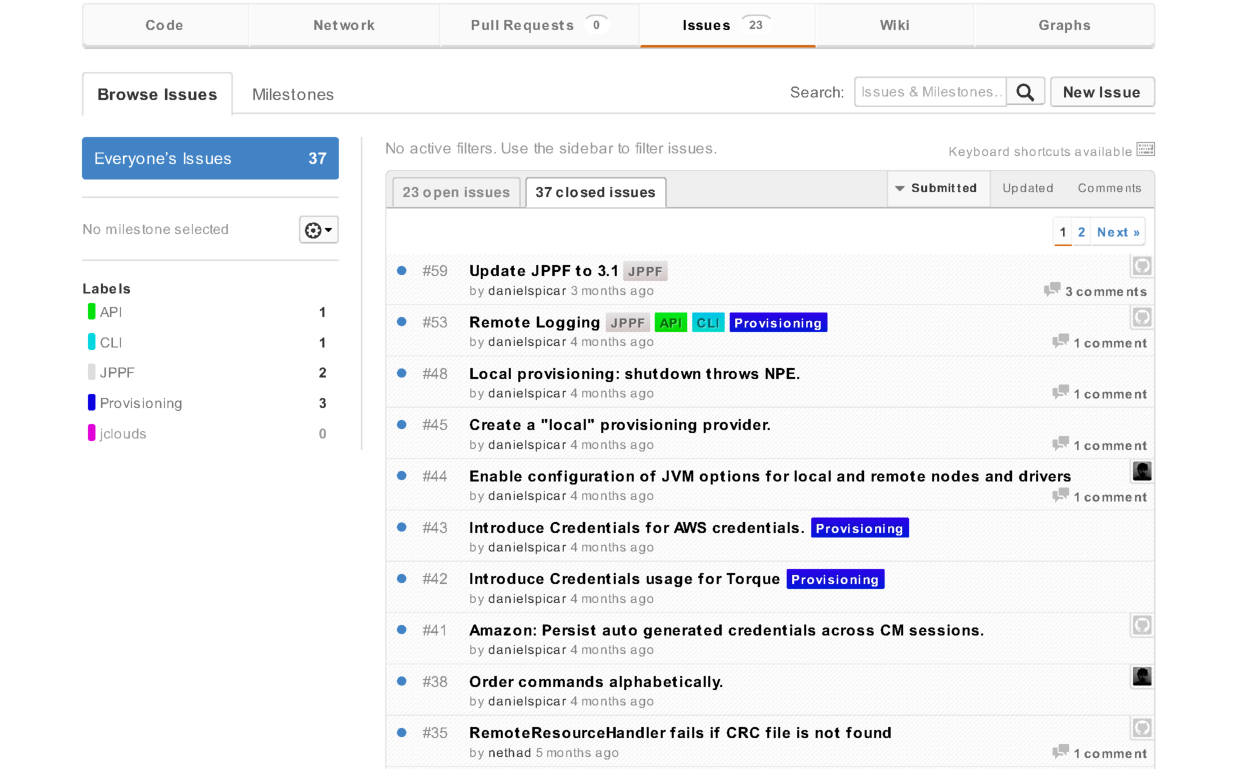
\includegraphics[scale=0.7]{images/github-issues.pdf}
\caption{Issue Management with GitHub}
\label{fig:issues}
\end{figure}

\section{Evaluation}
This sections summarizes the performance evaluation done with Clusterermeister. Areas of interest are the provisioning and deployment time (the time needed to make distributed Clustermeister nodes available and load user code on them) and job execution times (how Clustermeister can reduce the time needed to complete a computation job). 

\subsection{Provisioning and Deployment Time}

The time to provision the Clustermeister infrastructure strongly depends on the provisioning provider. When executing code on Clustermeister nodes another critical factor is the time to deploy user code and its dependencies on those nodes. 

\subsubsection{Troque Provisioning}
Torque cluster nodes are provisioned by queuing job requests on the queue management server. At some time the request is granted and a JPPF node is started. Provided the request has a high enough priority, this typically happens very quickly. Therefore the major time needed for provisioning falls to uploading the JPPF node executables and user configured libraries to the queue management server. The time for this depends on network latency, bandwidth and the size of configured libraries. However it is a one time investment only, provided the configuration is not changed and Clustermeister is not updated. Finally the JPPF node launches in about 5-8 seconds. For all these reasons the overall provisioning time is hard to predict but typically lies somewhere between 30 seconds and less than 10 seconds.

\subsubsection{Amazon Provisioning}
Amazon nodes can take significantly longer to be made available. While the same delays apply in respect to upload of binary data and launching a JPPF node, the binary files need to be uploaded to each instance and not only to the queue management server as in the Torque case. But the largest delay falls to the time needed for Amazon to make an EC2 instance available (loading a machine image, booting the machine, and configuring firewall and credentials on it). Creating a new instance and launching a Clustermeister node on it takes about 1 minute and 44 seconds on average (with a maximum measured time of 2:15 and a minimum of 1:30). Of course these numbers depend on the user configuration and network latency and bandwidth as well. On the other hand, launching a Clustermeister node on an already running instance takes merely about 8 seconds. To avoid  this long start up time, the Amazon provider performs node provisioning in parallel for all requested nodes.

\subsubsection{Code Deployment}
When a user executes code on Clustermeister, each class that is not available or out of date in a node's classpath, is loaded over the network from the user's classpath. This happens at runtime, one-by-one as the classes are loaded. Loading large amounts of classes or libraries in this way is very inefficient and may take several minutes. To mitigate this problem, Clustermeister offers the ability to pre-load libraries to nodes at provisioning time. Section \ref{appendix-general-configuration} describes how library pre-loading can be used.

\subsection{Execution Time}

Assessing execution time strongly depends on the nature of the computation task at hand. In the context of Clustermeister we are primarily interested in tasks that can be executed in parallel. This section uses the term \textit{job} to describe a single computation task, such as evaluating a list of numbers if they are primes. A job can then be split into a number of \textit{tasks} that can be executed in parallel (e.g. each number can be checked in parallel, provided there are enough resources). For the purposes of this evaluation two different kind of jobs were evaluated. Namely jobs that consists of a large number of trivial tasks with short execution time. And jobs that consist of a small number of long-running tasks. These two kinds of jobs behave very differently and as will be demonstrated, require different load-balancing (task distribution) algorithm for optimal performance. Clustermeister does not perform any load balancing but allows to configure the load balancing algorithm used by JPPF. The 
available choices are\footnote{http://www.jppf.org/doc/v3/index.php?title=Configuring\_a\_JPPF\_server\#Load-balancing}:

\begin{enumerate}
 \item \textbf{manual}: with this strategy, the user can provide a number of tasks that are executed on each node at most at the same time.
 \item \textbf{autotuned}: this strategy uses an adaptive heuristic algorithm based on the Monte Carlo algorithm.
 \item \textbf{proportional}: an adaptive deterministic algorithm based on the contribution of each node to the overall mean task execution time.
 \item \textbf{rl}: adaptive algorithm based on reinforcement learning.
 \item \textbf{NodeThreads}: each node receives at most n * m tasks, where n is the number of threads the node is configured to use, and m is a user-defined factor. 
\end{enumerate}

In the remainder of this section the data and conclusions obtained from this evaluation are presented.

\subsubsection{Job with many Short-Running Tasks}
\label{short-tasks}

For this evaluation the computation of an image of the Mandelbrot set\footnote{http://en.wikipedia.org/wiki/Mandelbrot\_set} has been chosen. The job creates a task for each row of the image and the task computes an array of color values. The computation of a single task is very fast (fractions of a second) but there are many tasks (600 tasks for an image with resolution 800 x 600). The evaluation was done with the Amazon EC2 provider on \textit{t1.micro} instances\footnote{http://aws.amazon.com/ec2/instance-types/}. The nodes were configured to use only one thread to computation so they could only execute one task at a time. For each run the job was configured to calculate the same part of the image to obtain comparable execution times. 

The first evaluation concentrated on the influence of the load balancing algorithm on execution times. This is not an evaluation of the load balancing algorithms but  an evaluation how much the execution time differs between the worst case and the best case. One part of the execution time measured is network overhead for sending the tasks to the nodes. JPPF can send multiple tasks in batches to nodes. The tasks are then queued on the node for execution but can not be sent to any other node any more. Another strategy is to queue the tasks on the JPPF server and distribute them to nodes as resources become available. To archive this behaviour, the NodeThreads algorithm has been chosen. Because each node has been configured with one thread only, the multiplicator (m) setting for this strategy determines the number of tasks that will be sent to each node in a batch (provided there are enough tasks to satisfy all upper limits).

The working hypothesis was that, assuming all nodes have equal computational resources, for tasks where the \textit{computation time} is much smaller than the \textit{network latency}, the optimal strategy is to distribute all tasks to all available nodes in one batch (see Tab. \ref{tab:mandelbrot-lb}). Contrary, the worst strategy would be to open a dedicated connection for every single task to send it to a node for execution (this equals batches of size 1). In this scenario there is a strong disproportion between network overhead and task computation time in favour of network overhead. The computation time of a task is simply too short to justify paying the overhead of establishing a dedicated connection over the network for every single task. Thus network overhead is expected to be the dominating factor in overall job execution time.

The hypothesis has been tested by running this evaluation on 6 nodes with the NodeThreads load balancing strategy and a multiplicator setting of 100 (best case) and 1 (worst case). The resulting execution times can be seen in Tab. \ref{tab:mandelbrot-lb-res}. It is very obvious that choosing the right load balancing strategy to minimize network latency is very important. The best case scenario is more than 14 times faster than the worst case scenario. And the difference is network overhead.

\begin{table}[h!]
\centering
\begin{tabular}{|c|c|}
\hline
\textbf{Tasks scheduled per node} & \textbf{Job Execution Time [ms]} \\ \hline
100 & 851 \\ \hline
1 & 12156 \\ \hline
\end{tabular}
\caption{Results of running the Mandelbrot set computation on 6 nodes with best case and worst case load balancing settings.}
\label{tab:mandelbrot-lb-res}
\end{table}

The other evaluation concentrated on the influence of number of nodes on execution time. More nodes equal more computation power but also more load balancing and network communication overhead. For this evaluation the load balancing strategy has been manually configured for optimal values under the assumption that each node has has equal resources (see Tab. \ref{tab:mandelbrot-lb}). Fig. \ref{fig:times-mandelbrot} shows the execution times for the Mandelbrot set job for 1 to 6 nodes. As expected the execution time is reduced for each node added. Using 6 nodes instead of 1 node, more than halves the execution time. However the decrease is not linear as the overhead increases with larger number of nodes.

\begin{table}[h!]
\centering
\begin{tabular}{|c|c|}
\hline
\textbf{\# of Nodes} & \textbf{Tasks scheduled per node} \\ \hline
1 & 600 \\ \hline
2 & 300 \\ \hline
3 & 200 \\ \hline
4 & 150 \\ \hline
5 & 120 \\ \hline
6 & 100 \\ \hline
\end{tabular}
\caption{Optimal load balancing settings for the Mandelbrot set evaluation. The goal is to distribute all tasks to all available nodes in one batch.}
\label{tab:mandelbrot-lb}
\end{table}

\begin{figure}[h]
\centering
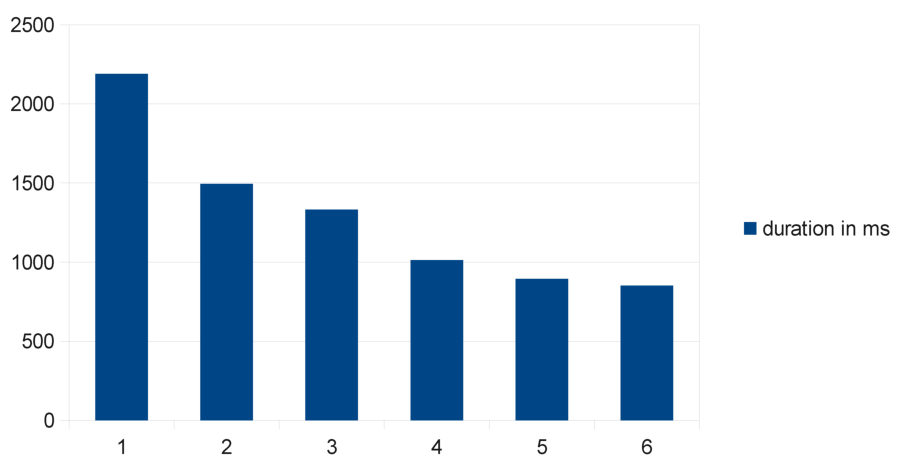
\includegraphics[scale=0.7]{images/amazon-duration.pdf}
\caption{Execution times for the Madelbrot set calcualtion job.}
\label{fig:times-mandelbrot}
\end{figure}

\subsubsection{Job with few Long-Running Tasks}

\begin{figure}[hptb]
\centering
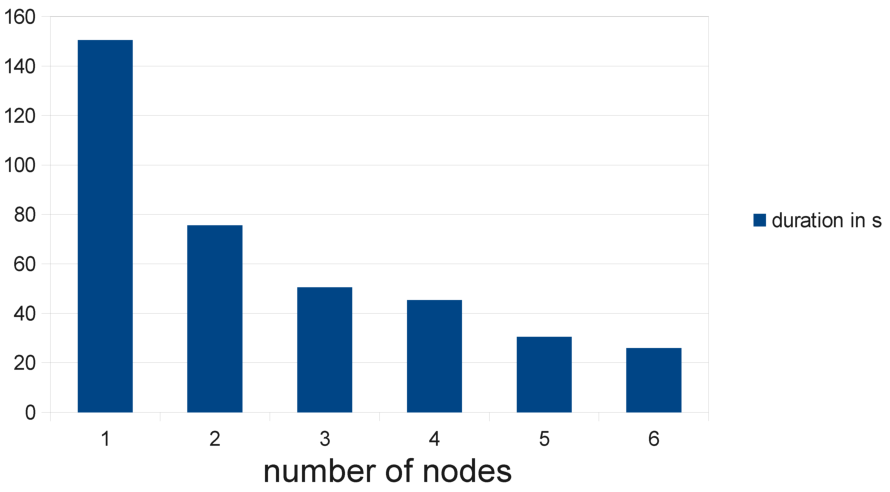
\includegraphics[scale=0.7]{images/long-running-duration.pdf}
\caption{Long-running tasks}
\label{fig:evaluation-long-running}
\end{figure}

In the simulation with long-running tasks, there were 30 tasks that had a duration of 5 seconds each. In fig. \ref{fig:evaluation-long-running}, the results of the simulation are shown in a chart. The number of nodes were increased from 1 to 6 for each simulation. Each node had one processing thread. In the simulation with 6 nodes, the optimal execution distributes 5 tasks for each node. Each task has a duration of 5 seconds, therefore the optimal execution time is 25 seconds. In the simulation, there was a duration of 25.928 seconds. Hence for long-running tasks, network overhead is neglectable and nodes are always fully utilized.

\subsubsection{Adaptive load balancing algorithms}

JPPF offers a number of adaptive load balancing strategies. These algorithms usually need to execute a number of jobs before they achieve good results. Their task distribution behaviour depends on statistics about a node's past performance and overall execution time. When very similar jobs (in terms of task number/execution time) are submitted repeatedly they often achieve close to optimal performance. However they can easily be thrown off when a job's tasks are very heterogeneous.

Another advantage of adaptive algorithms is that they can automatically tune the load balancing on a per node basis when the participating nodes have very different computation power. Therefore a weak node would receive less tasks than a strong node. This would be complicated or even impossible to achieve manually with the provided configuration options.

Figure \ref{fig:evaluation-learning} shows the job execution times for the Mandelbrot set evaluation (see section \ref{short-tasks}) when using the reinforced learning (rl) and the proportional load balancing strategies.

\begin{figure}[h]
\centering
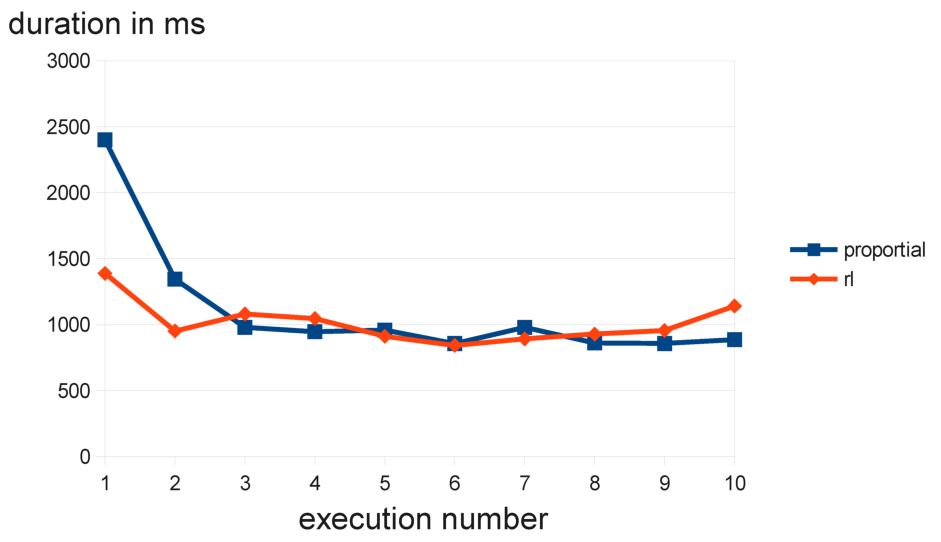
\includegraphics[scale=0.7]{images/learning-duration.pdf}
\caption{Execution times for the Mandelbrot set job for 10 runs with adaptive load balancing strategies.}
\label{fig:evaluation-learning}
\end{figure}

\subsubsection{Execution Time Conclusions}

The conclusions from this evaluations of execution times is that it is critical to choose the right load balancing strategy depending on the type of computation that is performed. When a task's computation time is much smaller than the network latency, it is important to minimize the task batches sent over the network by choosing an optimal batch size. When the tasks execution time is much larger than the network latency, it is best to not distribute tasks to nodes pre-maturely but instead queue the tasks on the server and send only small batches to nodes to prevent any node from becoming idle for a long time because no tasks are available for scheduling.

Finally, adaptive algorithms can be very good depending on the use case. If a user wants to execute only a single very long running job, adaptive algorithms are a bad idea. It is better to manually tune the load balancing settings. But if many jobs are going to be executed during a session, the adaptive algorithms will learn to perform well. Especially when the available nodes have very different computation power.

\newpage

\appendix

\section{User Manual}

\subsection{Tutorial}

\label{tutorial}

This tutorial shows the setup for a Java project. However, the steps discussed here should be applicable to other language environments running on the JVM, such as Scala. The code is deliberately kept simple, to show you how Clustermeister works and what a typical work-flow looks like. After that, however, it should be easy to build more complex projects.

\subsubsection{Setting Up A Java Project With Clustermeister API}

As a first step, you need to set up a Maven project. If you are not familiar with Maven, see their Maven in 5 Minutes intro\footnote{http://maven.apache.org/guides/getting-started/maven-in-five-minutes.html}. 
If you have not used Maven yet, do not worry, we provide you with the necessary configuration here. To start a new Maven project, enter:

\begin{lstlisting}[breaklines=true, backgroundcolor=\color{lbcolor}]
 mvn archetype:generate -DinteractiveMode=true -DarchetypeArtifactId=maven-archetype-quickstart
\end{lstlisting}

This is an interactive command which asks you for the mandatory Maven configuration. In our configuration, for the \texttt{groupId} you use \texttt{org.example.mycmproject} and for the \texttt{artifactId} you enter \texttt{helloworld}. You can choose other values, of course. For the version and package you just hit enter. After that, you are asked to confirm the values and you end up with this project structure:

\begin{lstlisting}[breaklines=true, backgroundcolor=\color{lbcolor}]
/helloworld
/helloworld/pom.xml
/helloworld/src/
/helloworld/src/main/
/helloworld/src/main/java/
/helloworld/src/main/java/org/example/mycmproject/
/helloworld/src/main/java/org/example/mycmproject/App.java
/helloworld/src/test/
/helloworld/src/test/java/
/helloworld/src/test/java/org/example/mycmproject/
/helloworld/src/test/java/org/example/mycmproject/AppTest.java
\end{lstlisting}

To use the Clustermeister API, you need to modify the \texttt{pom.xml} file and add the dependencies and the Clustermeister Maven Repository. After that, the \texttt{pom.xml} file should look like this:

\lstinputlisting[language=XML, numbers=left, showspaces=false, frame=single, breaklines=true, title=\lstname]{listings/pom.xml}

Now that you have created a new Maven project, you can prepare some nodes for code execution.

\subsubsection{Use The Clustermeister Command Line Interface To Run Nodes}

Before you can run any code, you need to deploy nodes that execute it. Clustermeister offers a "local" provider to run the code on the local machine. This is useful to test code and get familiar with the Clustermeister tools.

You need to get the command line client jar here\footnote{https://maven.ifi.uzh.ch/maven2/content/repositories/snapshots/com/github/nethad/clustermeister/cli/0.1-SNAPSHOT/} or build it yourself. If you choose to build it yourself, the jar lands in \texttt{clustermeister/cli/target/cli-0.1-SNAPSHOT.jar}.

To start the command line client, enter:

\begin{lstlisting}[breaklines=true, backgroundcolor=\color{lbcolor}]
java -jar cli-0.1-SNAPSHOT.jar -p local 
\end{lstlisting}

As you can see, we provide the command line argument \texttt{-p local}. With that, we specify the provider to use. Other providers would be \texttt{amazon} or \texttt{torque}. More information on the command line arguments may be obtained with the \texttt{-h} flag. After that, you will see the following logging output on the command line:

\begin{lstlisting}[breaklines=true, backgroundcolor=\color{lbcolor}]
29 May 2012 16:04:35,908 [INFO ][CLI]: Using configuration in /home/user/.clustermeister/configuration.yml or create file if it does not exist.
29 May 2012 16:04:35,911 [INFO ][CLI]: Using provider LOCAL
...
29 May 2012 16:04:36,100 [WARN ][CLI]: Configuration file "/home/user/.clustermeister/configuration.yml" does not exist, create default configuration.
... 
\end{lstlisting}

You have not yet created a configuration file yet, so a default configuration file is placed in\texttt{ ~/.clustermeister/configuration.yml}. More information on how to configure Clustermeister can be found in section \ref{configuration}. Since you choose the local provider, no configuration is necessary.

You should now be in the Clustermeister provisioning shell, recognizable by the \texttt{cm\$} prefix (If you do not see the prefix, press enter). You are now able to deploy nodes locally with

\begin{lstlisting}[breaklines=true, backgroundcolor=\color{lbcolor}]
cm$ addnodes 4 2
\end{lstlisting}

This deploys 4 nodes with 2 processing threads each. After a few seconds you should see

\begin{lstlisting}[breaklines=true, backgroundcolor=\color{lbcolor}]
...
29 May 2012 16:21:10,975 [INFO ][provisioning.local.JPPFLocalNode]: Start node with ./startNode.sh jppf-node-0.properties false false -Xmx32m
cm$ 29 May 2012 16:21:16,963 [INFO ][PROVISIONING]: Node connected 5BF598070A16C8BC0B6E5165940F0202
29 May 2012 16:21:17,322 [INFO ][PROVISIONING]: Node connected 32597083BD1422CA62CC94C56ED4DA76
29 May 2012 16:21:17,343 [INFO ][PROVISIONING]: Node connected 9E9907E000A0DD18F06275BE5CADAE90
29 May 2012 16:21:17,413 [INFO ][PROVISIONING]: Node connected 4A774FB8003209127A61BA48F9E5E3DD
\end{lstlisting}

The 4 nodes we deployed locally are now connected to the local driver. We are finally able to execute code on these nodes. Read on to learn how.

\subsubsection{Use The Clustermeister API To Execute Code On Nodes}

Now that you have deployed some nodes, you can start implementing the code. Change back to your newly created Maven project and add these two classes to the \texttt{helloworld/src/main/java/org/example/mycmproject/} folder:

\lstinputlisting[language=Java, numbers=left, showspaces=false, frame=single, breaklines=true, title=\lstname]{listings/HelloWorldCallable.java}

\lstinputlisting[language=Java, numbers=left, showspaces=false, frame=single, breaklines=true, title=\lstname]{listings/HelloWorld.java}

In the \texttt{main} method, you create a \texttt{Clustermeister} object and ask for all nodes that are currently provisioned. You iterate through all nodes and execute the \texttt{HelloWorldCallable} on each node. The \texttt{HelloWorldCallable} simply returns a \texttt{"Hello World!"} as a result. Back at the \texttt{main} method, you get a \texttt{ListenableFuture} (provided by the Google Guava Libraries\footnote{http://code.google.com/p/guava-libraries/}. To read more about the \texttt{ListenableFuture}, see their documentation\footnote{http://code.google.com/p/guava-libraries/wiki/ListenableFutureExplained}). With the \texttt{get()} method, you wait for the result and print it out. After all the "computations" are done (imagine a less ridiculous example with actual computations involved), you invoke \texttt{Clustermeister.shutdown()}.

\textbf{IMPORTANT:} Do not invoke \texttt{shutdown()} before all the results are returned! Code running on the nodes might dynamically load classes from your machine and the connection is torn down after the \texttt{shutdown()} command. In this example, you use the blocking \texttt{get()} command, so \texttt{shutdown()} is invoked after you received all results. But if you, for example, register callbacks on your futures and execute code meanwhile, the \texttt{finally} block might be invoked before your callbacks are executed, so keep this in mind!

You are finally able to run the code by executing the \texttt{HelloWorld} class. First you need to compile the two classes:

\begin{lstlisting}[breaklines=true, backgroundcolor=\color{lbcolor}]
mvn clean install
\end{lstlisting}

You should see

\begin{lstlisting}[breaklines=true, backgroundcolor=\color{lbcolor}]
...
[INFO] ------------------------------------------------------------------------
[INFO] BUILD SUCCESS
[INFO] ------------------------------------------------------------------------
...
\end{lstlisting}

at the end. If the build succeeded, we can start our HelloWorld class with:

\begin{lstlisting}[breaklines=true, backgroundcolor=\color{lbcolor}]
mvn exec:java -Dexec.mainClass="org.example.mycmproject.HelloWorld"
\end{lstlisting}

In the output, you should see:

\begin{lstlisting}[breaklines=true, backgroundcolor=\color{lbcolor}]
...
[INFO ][API] - Provisioning returned 4 nodes.
Node 9E9907E000A0DD18F06275BE5CADAE90, result: Hello world!
Node 32597083BD1422CA62CC94C56ED4DA76, result: Hello world!
Node 5BF598070A16C8BC0B6E5165940F0202, result: Hello world!
Node 4A774FB8003209127A61BA48F9E5E3DD, result: Hello world!
[INFO] ------------------------------------------------------------------------
[INFO] BUILD SUCCESS
[INFO] ------------------------------------------------------------------------
...
\end{lstlisting}

When you are finished, you can shut down the locally provisioned nodes. Change to the Clustermeister CLI and type:

\begin{lstlisting}[breaklines=true, backgroundcolor=\color{lbcolor}]
cm$ shutdown
\end{lstlisting}

When shutdown completed, type exit to leave the CLI.

And that is all. You have set up a new Maven project, configured with the Clustermeister API. You have set up 4 local nodes and executed a Hello World example on them. To see more elaborate examples, check out the Clustermeister Examples repository\footnote{https://github.com/nethad/clustermeister-examples}.

\subsection{Clustermeister API}

The Clustermeister API offers 4 different ways to execute code on provisioned nodes. These are:

\begin{itemize}
 \item via an ExecutorService\footnote{http://docs.oracle.com/javase/6/docs/api/java/util/concurrent/ExecutorService.html}
 \item execute code on addressable nodes
 \item with Clustermeister Jobs and Tasks
 \item via the native JPPF interface\footnote{http://jppf.org/}
\end{itemize}

All of these are discussed in the following.

Further, you can find functional examples in the Clustermeister Examples Repository\footnote{https://github.com/nethad/clustermeister-examples}.

\subsubsection{ExecutorService}

The \texttt{ExecutorService} is an Java interface and therefore offers interoperability with existing projects.

You can request an ExecutorService with \texttt{Clustermeister.getExecutorService(ExecutorServiceMode)}. The \texttt{ExecutorServiceMode} enables you to define task scheduling preferences:

\begin{itemize}
 \item \texttt{ExecutorServiceMode.standard()} executes Callabes/Runnables immediately.
 \item \texttt{ExecutorServiceMode.timeConstraint(long timeout)} bundles Callables/Runnables and executes them after the given timeout (in milliseconds)
 \item \texttt{ExecutorServiceMode.batchSizeContraint(int batchSize)} bundles Callables/Runnables and executes them after the given count.
 \item \texttt{ExecutorServiceMode.timeoutAndBatchSizeContraint(long timeout, int batchSize)} bundles Callables/Runnables and executes them if either a timeout (in milliseconds) occurs or the given count is reached, depending on what happens first.
\end{itemize}

Since Clustermeister wraps a JPPFExecutorService, more information can be found in the JPPFExecutorService Javadoc\footnote{http://jppf.org/api-3/org/jppf/client/concurrent/JPPFExecutorService.html}.

\subsubsection{Addressable Nodes}

With an ExecutorService and the Clustermeister Jobs and Tasks, you cannot control on which nodes your tasks are executed. If you need this flexibility, you can choose your nodes by calling \texttt{Clustermeister.getAllNodes()} which returns you a list of ExecutorNodes. An ExecutorNode offers node characteristics with \texttt{ExecutorNode.getCapabilities()} and an execution handle via \texttt{ExecutorNode.execute(Callable)}.

\subsubsection{Clustermeister Jobs and Tasks}

Clustermeister Jobs are a nice way to bundle tasks that belong together. It further offers to attach read-only data to a Job that can be used by all Tasks.

To create a Job, you call \texttt{JobFactory.create(String name, Map<String, Object> jobData)}. Both are optional, but the \texttt{jobData} enables you to add arbitrary data to your job with a given key. To read this data, you extend a \texttt{Task} which offers you \texttt{Task.getValue(String key)}.

To add a Task to a Job, you simply call \texttt{Job.addTask(Task)} and then execute the Job with \texttt{Clustermeister.executeJob(Job)}. The \texttt{executeJob()} method is blocking. If you want to submit your job asynchronously, you can either use \texttt{executeJobAsync()}, which returns you a ListenableFuture\footnote{http://code.google.com/p/guava-libraries/wiki/ListenableFutureExplained} with the list of results or the more fine-grained \texttt{executeJobAsyncTasks()}, which returns a list of ListenableFutures. Every Future belongs to a task and the Future completes as soon as the corresponding task is finished, so you do not need to wait for all the tasks to be finished.

\subsubsection{Native JPPF Interface}

If all the methods above do not offer you enough flexibility, you can still access the unterlying \texttt{JPPFClient}, which Clustermeister uses internally. For more information on this, see the JPPF documentation\footnote{http://jppf.org/doc/v3/index.php?title=JPPF\_3.x\_Documentation}.

\subsection{Command Line Interface}

The Clustermeister command line client is the user interface to interact with the provisioning module. It sets up the provisioning infrastructure needed to communicate with and deploy Clustermeister nodes.

The Tutorial in section \ref{tutorial} describes how to obtain and run the command line interface (CLI).

This page documents the CLI capabilities and especially the different capabilities of the supported three providers (Torque, Amazon, Local).

The basic capabilities of the CLI include command completion and listing of available commands as well as printing of usage instructions for these commands.

\subsubsection{Commands supported by all providers}


\begin{table}[h]
\centering
\begin{tabular}{|l|l| p{7cm}|}
\hline
\textbf{Command} & \textbf{Arguments} & \textbf{Description} \\ \hline
help & none & Prints a list of available commands and a short description. \\ \hline
shutdown & none & Shuts down all running Clustermeister nodes and the provisioning infrastructure. \\ \hline
exit & none & Quits the CLI. \\ \hline
\end{tabular}
\end{table}

\textbf{IMPORTANT}: If you call the \texttt{exit} command before calling the \texttt{shutdown} command you will have to shut down the running Clustermeister by other means than the CLI. Also properly exiting the CLI requires the \texttt{shutdown} command followed by the \texttt{exit} command. Note that after the \texttt{shutdown} command has been issued, the CLI will be in an inconsistent state and can not be used to deploy nodes anymore. The only command that should be used then is the exit command. We understand that this is confusing and a solution is being worked on.


\subsubsection{Troque Provider}

This provider supports PBS/TORQUE setups by logging in to a queue management machine via SSH and issuing \texttt{qsub} commands. To use the torque provider start the CLI with the \texttt{-p torque} argument.

The commands are described in table \ref{tab:torqueprovider}.

\begin{table}[h]
\centering
\begin{tabular}{|l| p{3cm} | p{6cm}|}
\hline
\textbf{Command} & \textbf{Arguments} & \textbf{Description} \\ \hline
state & none & Lists the currently running nodes with their node ID and number of processing threads. Also prints the number of currently running nodes. \\ \hline
addnodes & [number of nodes] [processing threads per node] & Starts new Clustermeister nodes. You can specify how many processing threads a node should use. Typically the total number of processing nodes per physical machine should be approximately the number of CPUs or CPU cores. \\ \hline
removenode & node ID... & Shuts down the listed node IDs. \\ \hline
\end{tabular}
\caption{Torque provider commands}
\label{tab:torqueprovider}
\end{table}

\subsubsection{Amazon Provider}

This provider supports Amazon EC2. To use the amazon provider start the CLI with the -p amazon argument.

The commands are described in table \ref{tab:amazonprovider}.

\begin{table}[h]
\centering
\begin{tabular}{|l| p{3cm} | p{6cm}|}
\hline
\textbf{Command} & \textbf{Arguments} & \textbf{Description} \\ \hline
state & none & Lists all currently running nodes and their properties (node ID, IP addresses, amazon instance ID). \\ \hline
addnodes & [number of nodes] [profile name] & Starts the specified number of nodes with the specified (and previoulsy configured) node profile. See Configuration for details. \\ \hline
get instances & -v (optional, to print more details) & Lists all EC2 instances associated to the configured AWS Account. \\ \hline
get keypairs & none & Lists all key pair credentials known to Clustermeister for this AWS Account or configured in the configuration file. See Configuration for details. \\ \hline
get profiles & none & Lists all configured instance profiles and their properties. See Configuration for details. \\ \hline
instance resume & EC2 instance ID & Start a suspended AWS EC2 instance. \\ \hline
instance suspend & EC2 instance ID & Shutdown a running AWS EC2 instance. \\ \hline
instance terminate & EC2 instance ID & Shutdown and delete an AWS EC2 instance. \\ \hline
removenode & [shutdown state] [node ID...] & Remove a Clustermeister node and put the EC2 instance into the specified shutdown state. \\ \hline
startnode & EC2 instance ID & Start a Clustermeister node on a suspended or running EC2 instance. \\ \hline
\end{tabular}
\caption{Amazon provider commands}
\label{tab:amazonprovider}
\end{table}


\subsubsection{Local Provider}

The local provider has very limited capabilities and is only intended for local testing. The local provider is the default provider but it can be explicitly chosen by launching the CLI with the \texttt{-p local} argument.

The commands are described in table \ref{tab:localprovider}.

\begin{table}[h]
\centering
\begin{tabular}{|l| p{3cm} | p{6cm}|}
\hline
\textbf{Command} & \textbf{Arguments} & \textbf{Description} \\ \hline
state & none & Prints the number of currently running Clustermeister nodes. \\ \hline
addnodes & [number of nodes] [processing threads per node] & Starts new Clustermeister nodes. You can specify how many processing threads a node should use. Typically the total number of processing nodes per physical machine should be approximately the number of CPUs or CPU cores. \\ \hline
\end{tabular}
\caption{Local provider commands}
\label{tab:localprovider}
\end{table}


\subsection{Configuration}

\label{configuration}

The default configuration is expected at \texttt{~/.clustermeister/configuration.yml} (that is \texttt{/home/username/.clustermeister/configuration.yml} for Linux and \texttt{/Users/username/.clustermeister/configuration.yml}. The configuration files are written in YAML.

\subsubsection{High-level structure}

The configuration file has different sections, these are the top-level keys:

\begin{itemize}
 \item \textbf{amazon}: Configuration related to the amazon provider.
 \item \textbf{torque}: Configuration related to the torque provider.
 \item \textbf{preload}: Configuration independent of any provider, related to library-preloading for nodes (to speed up code execution by avoiding remote class-loading).
 \item \textbf{jvm\_options}: JVM fine-tuning for the local provider and (remote) nodes.
 \item \textbf{logging}: Logging configuration (currently only for remote logging from nodes).
\end{itemize}

The configuration file is structured like this:

\lstinputlisting[numbers=left, showspaces=false, frame=single, breaklines=true]{listings/config_structure.yaml}

\subsubsection{Provider Configuration: Amazon}

\paragraph{AWS Credentials}

In order to access the EC2 API, Clustermeister requires the configuration the Access Key ID and the Secret Key\footnote{http://docs.amazonwebservices.com/AWSEC2/latest/UserGuide/using-credentials.html\#using-credentials-access-key}.

\begin{lstlisting}[breaklines=true, frame=single]
access_key_id: <Access Key ID> 
secret_key: <Secred Key>
\end{lstlisting}

\paragraph{Instance Profiles}

Because it would be very complicated to configure EC2 Instances on the command line each time, Clustermeister uses configured instance profiles that define the capabilities, credentials and location of EC Instances.

A user can define an arbitrary number of profiles with custom, user-defined names.

Currently Clustermeister supports these properties for instance profiles:

% \begin{table}[h]
% \centering
\begin{longtable}{|l| p{6cm} | p{3cm}|}
\hline
Property & Description & Default\\ \hline
type & AWS EC2 Instance Type. Specification and valid values (check 'API Name') can be found here\footnote{http://aws.amazon.com/ec2/instance-types/}. & none (required)\\ \hline
region & AWS EC2 Region. Valid values (check 'Endpoint' which has the format 'ec2.<region>.amazonaws.com') can be found here\footnote{http://docs.amazonwebservices.com/general/latest/gr/rande.html\#ec2\_region}. See also Using Regions and Availability Zones\footnote{http://docs.amazonwebservices.com/AWSEC2/latest/UserGuide/using-regions-availability-zones.html}. & none (required)\\ \hline
zone & AWS EC Availability Zone. See also Using Regions and Availability Zones. & no preference (random assignment)\\ \hline
ami\_id & Specifies the AMI (Amazon Machine Image) to use by its ID. & the highest version of the Amazon Linux AMI\\ \hline
keypair & A reference to a configured keypair name (see section of Keypairs). This keypair is used for SSH access to instances that use this profile. If no keypair is configured, Clustermeister generates one automatically for internal use. However is you desire to access the instance via SSH yourself you should configure a keypair. & auto-generated credentials\\ \hline
shutdown\_state & The state to which the instance is put when it is shut down. Valid values are: 'terminated' (the instance is deleted and can not be started anymore), 'suspended' (the instance can be started again) and 'running' (the node is removed from clustermeister but the EC2 instance continues running). & suspended\\ \hline
group & Affects the name of instances (e.g. in the EC2 Console) and is required for spot instances that launch and shut down together. & clustermeister\\ \hline
spot\_price & If a spot price (a float value in US Dollar) is set, the instances are started as spot instances. See also Amazon EC2 Spot Instances\footnote{http://aws.amazon.com/ec2/spot-instances/}. & none (required for spot instances)\\ \hline
spot\_request\_type & Spot instances can get terminated, for example when the spot price goes beyond the configured spot price. If a request duration (see 'spot\_request\_valid\_from' and 'spot\_request\_valid\_to') is configured, this option determines if the spot instances are restarted again provided the circumstances allow for it (e.g. spot price is below spot price). Valid values are 'one\_time' (when instances get terminated they do not restart) and 'persistent' (restart terminated instances for the duration of the request). & one\_time\\ \hline
spot\_request\_valid\_from & From which point in time a spot request is active. Valid values are formatted according to following pattern: yyyy-MM-dd HH:mm & none (any time)\\ \hline
spot\_request\_valid\_to & Until which point in time a spot request is active. Valid values are formatted according to following pattern: yyyy-MM-dd HH:mm & none (any time) \\ \hline
placement\_group & Specifies a user-defined unique name for a cluster placement group. See also What is a cluster placement group?\footnote{http://aws.amazon.com/ec2/faqs/\#What\_is\_a\_cluster\_placement\_group}. & none (required for cluster instances) \\ \hline
\end{longtable}
% \end{table}

\paragraph{Example configurations}

Here are a few template configurations:

\lstinputlisting[numbers=left, showspaces=false, frame=single, breaklines=true]{listings/example_configurations.yaml}

\paragraph{Keypair (Credentials)}

Generally Clustermeister does not need to be configured with custom credentials for instance profiles. It can generate its own credentials and access these nodes. However, custom AMIs may require different credentials or if the user wants to log into an instance with SSH the auto generated credentials may not work.

In such a case it is possible to supply custom credentials or use credentials configured in the AWS EC2 Console. The credentials have to be configured and referenced from the instance profile configurations (see property 'keypair').

A user can define an arbitrary number of keypairs with custom, user-defined names.

Note: Currently custom keypairs have to be password-less because Clustermeister does not support private key passwords.

\lstinputlisting[numbers=left, showspaces=false, frame=single, breaklines=true]{listings/amazon_keypairs.yaml}

\paragraph{Example Amazon Configuration}

This is a full Amazon provider configuration example:

\lstinputlisting[numbers=left, showspaces=false, frame=single, breaklines=true]{listings/example_amazon_configuration.yaml}

\subsubsection{Torque Configuration}

The Torque configuration is relatively simple. Each node that is deployed to a Torque cluster is a new Torque job. It is assumed that Torque jobs are started via SSH on a job submission server and with the Torque \texttt{qsub} command. Here is a sample configuration with comments:

\lstinputlisting[numbers=left, showspaces=false, frame=single, breaklines=true]{listings/example_torque_configuration.yaml}

\textbf{IMPORTANT}: it is assumed that the private key does not require a password, because node deployments have to be automated. Furthermore, SSH logins with passwords are not supported by Clustermeister.

\subsubsection{General Configuration}

\label{appendix-general-configuration}

This sections contains configurations that are independent of providers.

\paragraph{Preloading}

When executing code on remote, distributed nodes, there are are usually numerous dependencies. Although these dependencies can be dynamically loaded over the network, it can easily take a few minutes until all classes are loaded and any code is actually executed. This is cumbersome and the preloading configuration circumvents this by uploading dependency jar files at deploy time. The preloading configuration specifies which jar files need to be preloaded.

Since Clustermeister supports Maven natively, you can specify a \texttt{pom.xml} file from which dependencies are extracted. A configuration could look like this:

\lstinputlisting[numbers=left, showspaces=false, frame=single, breaklines=true]{listings/preload_configuration.yaml}

With \texttt{excludes} you can specify dependencies that are ignored for preloading. To manually add dependencies (this is possible without specifying a pom.xml), you can add \texttt{artifacts}. The string for manually added dependencies are structured as: 

\begin{lstlisting}[breaklines=true]
groupId:artifactId:version
\end{lstlisting}

If you wanted to add the Google Guava Libraries in version 12.0, the notation would be:

\begin{lstlisting}[breaklines=true]
"com.google.guava:guava:12.0"
\end{lstlisting}

If you specify dependencies which are not in the Maven Central Repository, you can add other repositories:

\lstinputlisting[numbers=left, showspaces=false, frame=single, breaklines=true]{listings/preload_repo_configuration.yaml}

With these configuration options, you can significantly speed up your code execution time.

\paragraph{JVM Options}

In the JVM Options configuration, you can specify JVM Options for the local driver and (remote) nodes. This enables you, for example, to fine-tune memory management. See the documentation\footnote{http://docs.oracle.com/javase/6/docs/technotes/tools/windows/java.html} for more information on JVM Options.

The most common option would probably be:

\begin{lstlisting}[breaklines=true, frame=single]
jvm_options:
  local_driver: "-Xmx500m"
  node: "-Xmx300m"
\end{lstlisting}

This sets the maximum size of the memory allocation pool to 500 megabytes for the local driver, and to 300 megabytes for each node. You can add more options, separated with spaces, just as you would on the command line.

\paragraph{Logging}

With the logging configuration you can configure remote logging from nodes. Remote logging means that you can see log statements from Clustermeister nodes in the CLI and local log files.

The logging configuration currently supports the properties defined in table \ref{tab:loggingproperties}

\begin{table}[h]
\centering
\begin{tabular}{| l | p{9cm} | l |}
\hline
\textbf{Property} & \textbf{Description} & \textbf{Default} \\ \hline
remote & This property can either be 'true' or 'false' and turns remote logging on or off. & false \\ \hline
remote\_port & The local TCP port on which a server process listens for incoming remote logging statements. Must be a valid TCP port number (from 0 to 65536) and should not be used by any other process. & 52321 \\ \hline
level & Specifies the log level on remote nodes (irrespective of remote logging being used or not). Valid values are: TRACE, DEBUG, INFO, WARN and ERROR. & INFO \\ \hline
\end{tabular}
\caption{Logging properties}
\label{tab:loggingproperties}
\end{table}

Here is an example configuration:

\begin{lstlisting}[breaklines=true, frame=single]
logging:
  node:
   remote: true
   remote_port: 54451
   level: INFO
\end{lstlisting} 



\end{document}
